
\chapter{Validierung}

\subsection{Versuchsaufbau}

\begin{figure}
    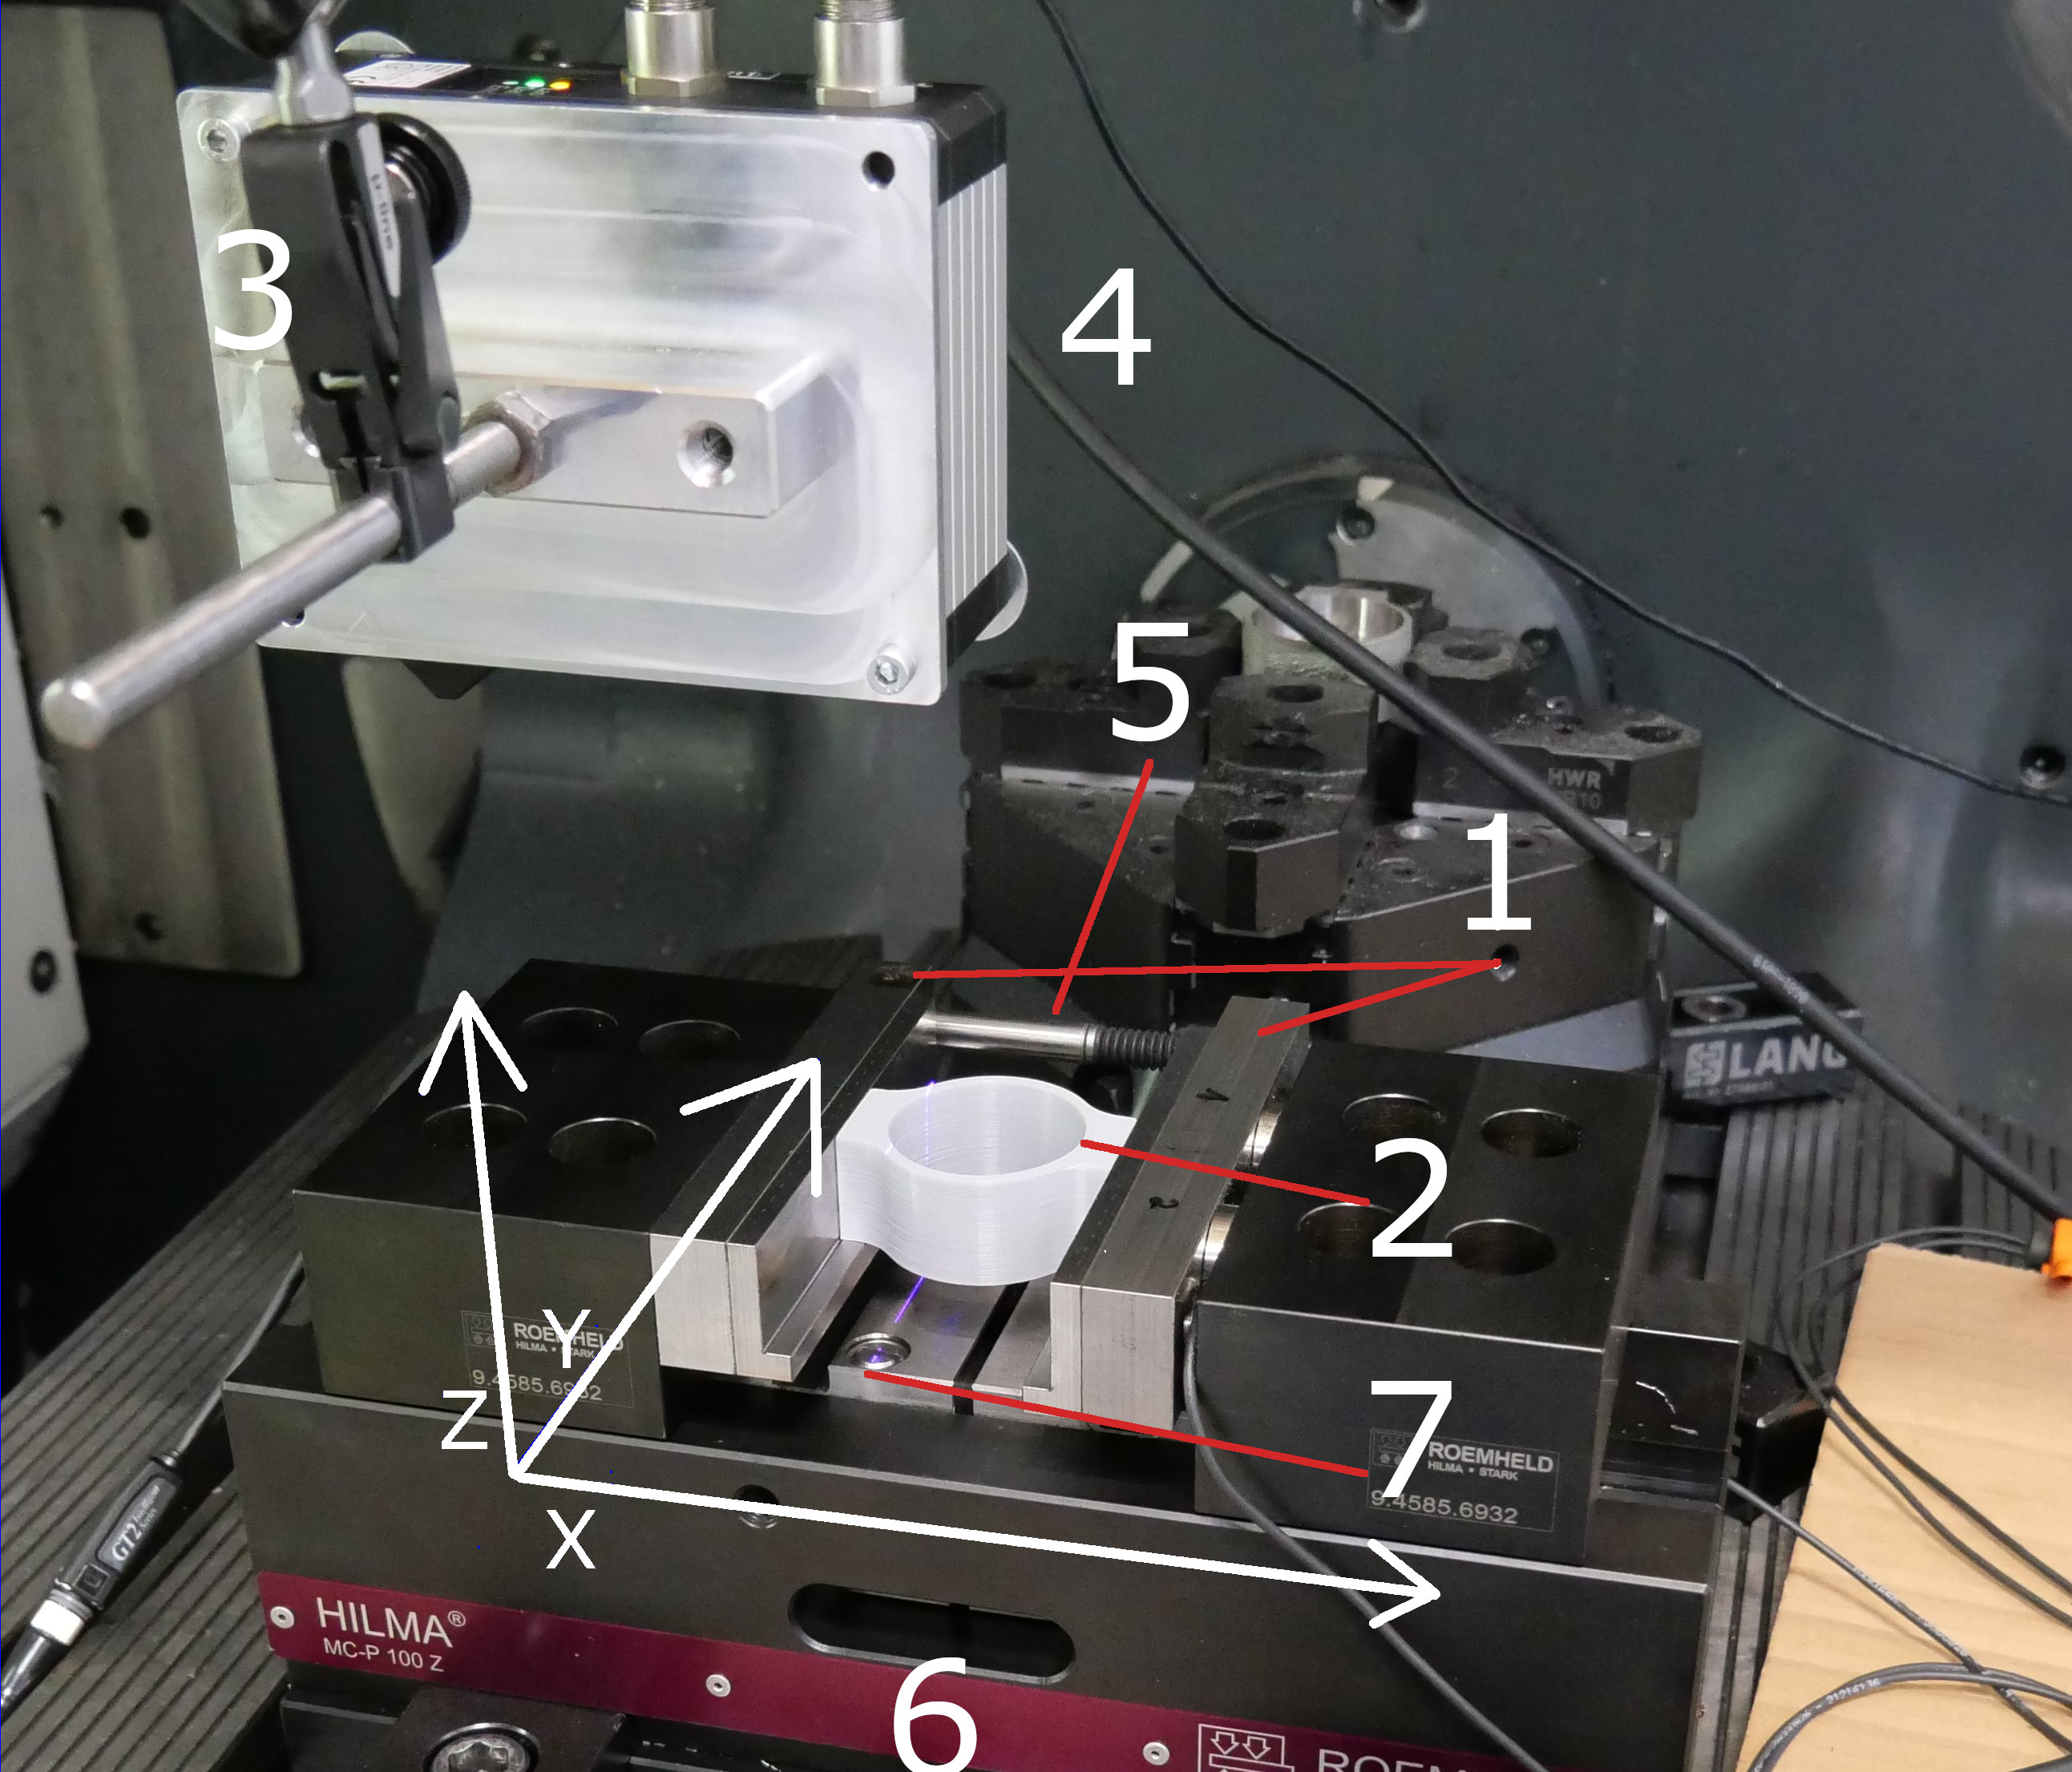
\includegraphics[width=0.6\textwidth]{images/versuchsaufbau_foto.png.JPG}
    \caption{Versuchsaufbau}
    \label{fig:versuchsaufbau}
\end{figure}

In Abbildung \ref{fig:versuchsaufbau} ist der Versuchsaufbau zur Datenerfassung 
zu sehen. Alle wichtigen Bestandteile sind nummeriert. Es folgt eine kurze Benennung
aller vorhandenen und notwendigen Teile:\\
1: Schraubstock Backen\\
2: Demonstratorbauteil\\
3: Scannerhalterung\\
4: Scanner LLT 30x0-25\\
5: Verschiebungsmesser\\
6: Laserlinie (Lila)\\
7: Schraubstock mit Kraftmesser\\
X: x-Achse\\
Y: y-Achse\\
Z: z-Achse\\

Der Scanner ist an dem Werkzeugkopf einer CNC-Fräse befestigt und wird 
in Richtung der X und Y Achse verschoben. So kann von dem kompletten Bauteil eine 
Pointcloud aufgenommen werden.

\section{Zusätzliche Messinstrumente}

Zusätzlich zu dem Scanner werden noch mit weiteren Messinstrumente Daten erfasst.
In Abbildung \ref{fig:versuchsaufbau} unter der Nummer 5 ist ein mechanischer 
Verschiebungsmesser zu sehen. Dieser misst die Verschiebung der Backen des 
Schraubstocks. Der Schraubstock misst zusätzlich mit viel Kraft die Backen 
aufeinander pressen.

Hierzu wird die piezoelektrische Kraftmesstechnik verwendet.
Bei Krafteinwirkung auf Piezokristalle (z. B. Quarz, Bariumtitanat, BaTiO3) 
werden im Kristallgitter negative gegen positive Gitterpunkte
verschoben, sodass an den Kristalloberflächen
Ladungsunterschiede Q als Funktion der Kraft F
gemessen werden.
Piezoelektrische Kraftaufnehmer sind mechanisch sehr steif, 
sie erfordern Ladungsverstärker
zur Messsignalverarbeitung und sind hauptsächlich zur Messung dynamischer Vorgänge
mit einer kleineren Frequenz als 1 Hz geeignet. \cite{Czichos.2020}. 
Diese Kraftmesstechnik ist 
für unseren Einsatzzweck gut geeignet da sie eine hohe Empfindlichkeit bietet 
und in vielfältigen Formen und Größen hergestellt werden kann. Zur Aufbereitung 
der Ladung, die der piezoelektrische Sensor, liefert wurde ein Ladungsverstärker 
eingesetzt.\cite{Schwartz.2006}
Dieser ist in Spannungsverstärker ist in Abbildung \ref{fig:taster} unten zu sehen.

\begin{figure}[b]
    \includegraphics[width=0.4\textwidth]{images/taster.JPG}
    \caption{Taster}
    \label{fig:taster}
\end{figure}

\begin{figure}[b]
    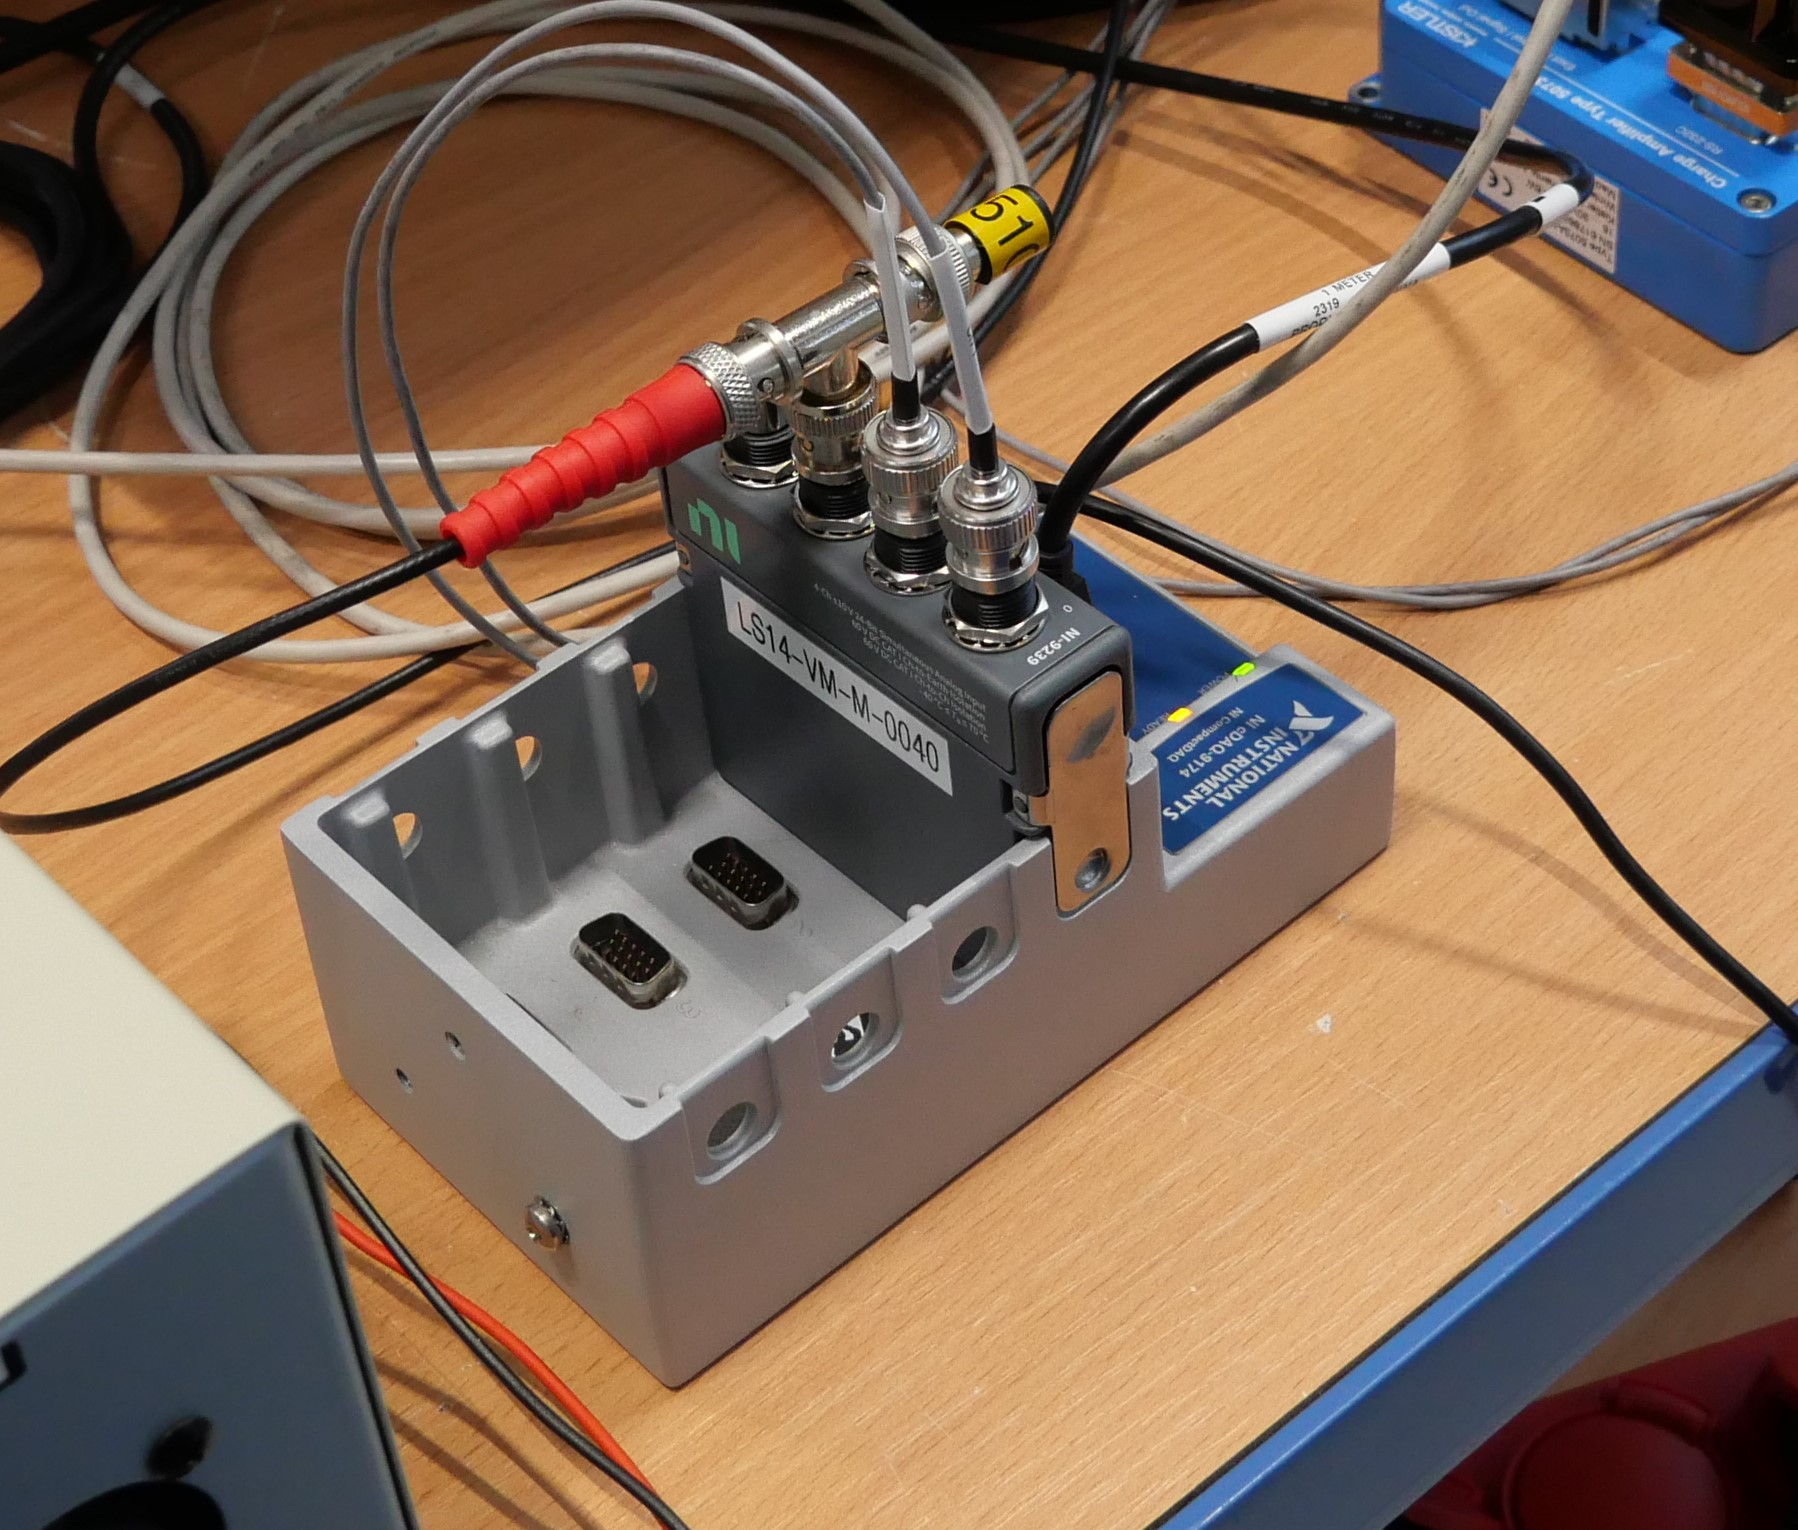
\includegraphics[width=0.4\textwidth]{images/piezoelektrische.JPG}
    \caption{Spannungswandler}
    \label{fig:piez}
\end{figure}

Damit die Scanner Ergebnisse überprüft werden können,
wird die Bauteilgeometrie zusätzlich nach dem Scanvorgang noch mit einem Taster
abgetastet. Hierfür wird der Werkzeugkopf gewechselt und der Scanner entfernt.
Dann wird der Taster in die CNC-Maschine eingesetzt und das Bauteil abgetastet.
In Abbildung \ref{fig:taster} ist das Tasterwerkzeug zu sehen. Die rote Kugel 
am Ende des Tasters erkennt, sobald eine Berührung zu dem Bauteil erfolgt ist 
und benachrichtigt den Steuerungsrechner. Dieser speichert die aktuelle Position 
dann in einer Protokolldatei.

